% This is text associated with the open textbook "Open Electromagnetics"
% See immediately below for author, date
% This work is licensed under the Creative Commons Attribution-ShareAlike 4.0 International License. (CC BY-SA 4.0) 
% To view a copy of the license, visit http://creativecommons.org/licenses/by-sa/4.0/

%ORB TITLE Input Impedance for Open- and Short-Circuit Terminations
%ORB AUTHOR 0        # S.W. Ellingson, Virginia Tech (ellingson@vt.edu)
%ORB DATE 20180802   # yyyymmdd
%ORB ABSTRACT Input Impedance for Open- and Short-Circuit Terminations 

\label{m0088_Input_Impedance_for_Open_and_Short_Circuit_Terminations}  % <-- Must match name of this file and module directory name.  Don't mess with this!
\index{transmission line!input impedance|(}

Let us now consider the input impedance of a transmission line that is terminated in an open- or short-circuit.
Such a transmission line is sometimes referred to as a \emph{stub}.
\index{stub!definition}
\index{transmission line!stub|see{stub}}
First, why consider such a thing?  
From a ``lumped element'' circuit theory perspective, this would not seem to have any particular application.
However, the fact that this structure exhibits an input impedance that depends on length (Section~\ref{m0087_Input_Impedance_of_a_Terminated_Lossless_Transmission_Line}) enables some very useful applications.

First, let us consider the question at hand: 
What is the input impedance when the transmission line is open- or short-circuited? 
For a short circuit, 
\index{short circuit}
\index{stub!short circuit}
$Z_L=0$, $\Gamma=-1$, so we find 
%
\begin{flalign}
Z_{in}(l) &= Z_0 \frac{ 1 + \Gamma e^{-j2\beta l} }{  1 - \Gamma e^{-j2\beta l} } \nonumber \\
          &= Z_0 \frac{ 1 - e^{-j2\beta l} }{  1 + e^{-j2\beta l} } 
\end{flalign}
%
Multiplying numerator and denominator by $e^{+j\beta l}$ we obtain%
\begin{equation}
Z_{in}(l) = Z_0 \frac{ e^{+j\beta l} - e^{-j\beta l} }{  e^{+j\beta l} + e^{-j\beta l} } 
\end{equation}
%
Now we invoke the following trigonometric identities:
%
\begin{flalign}
\cos\theta &= \frac{1}{2}\left[ e^{+j\theta} + e^{-j\theta} \right] \\
\sin\theta &= \frac{1}{j2}\left[ e^{+j\theta} - e^{-j\theta} \right] 
\end{flalign}
%
Employing these identities, we obtain:
%
\begin{equation}
Z_{in}(l) = Z_0 \frac{ j2\left(\sin\beta l\right) }{ 2\left(\cos\beta l\right)  } 
\end{equation}
%
and finally:
%
\begin{equation}
\boxed{
Z_{in}(l) = +jZ_0 \tan \beta l 
}
\label{m0088_eZstubSC}
\end{equation}

Figure~\ref{m0088_fZin}(a) shows what's going on.
As expected, $Z_{in}=0$ when $l=0$, since this amounts to a short circuit with no transmission line.
Also, $Z_{in}$ varies periodically with increasing length, with period $\lambda/2$. This is precisely as expected from standing wave theory (Section~\ref{m0086_Standing_Waves}).
What is of particular interest now is that as $l\rightarrow\lambda/4$, we see $Z_{in}\rightarrow\infty$. Remarkably, the transmission line has essentially transformed the short circuit termination into an open circuit!  
%
\begin{figure}
\begin{center}
\pdftooltip{{  % note double braces
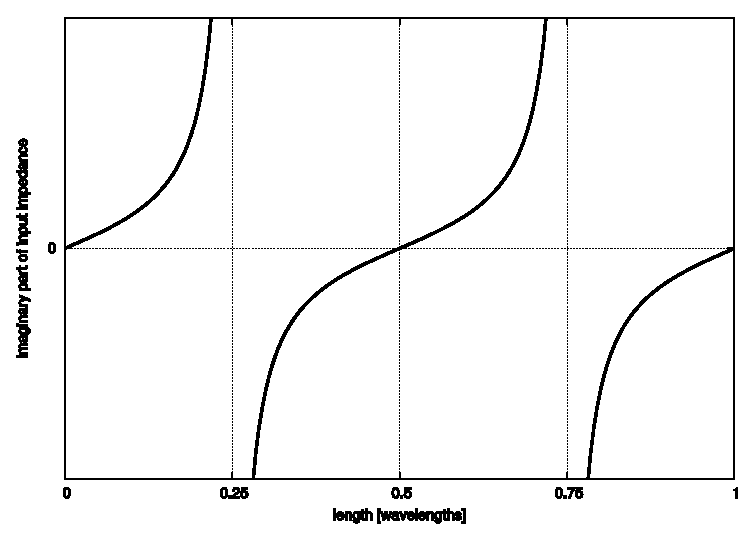
\includegraphics[width=\columnwidth]{modules/m0088_fZinSC.eps}
}}{A plot of the imaginary part of the input impedance (no scale shown) versus length from zero to 1 wavelength.  The plot has the form of the tangent function, with zeros at 0, 0.5, and 1 wavelength and positive asymptotes at 0.25 and 0.75 wavelengths.}\\
(a) Short-circuit termination ($Z_L=0$).\\~\\
\pdftooltip{{  % note double braces
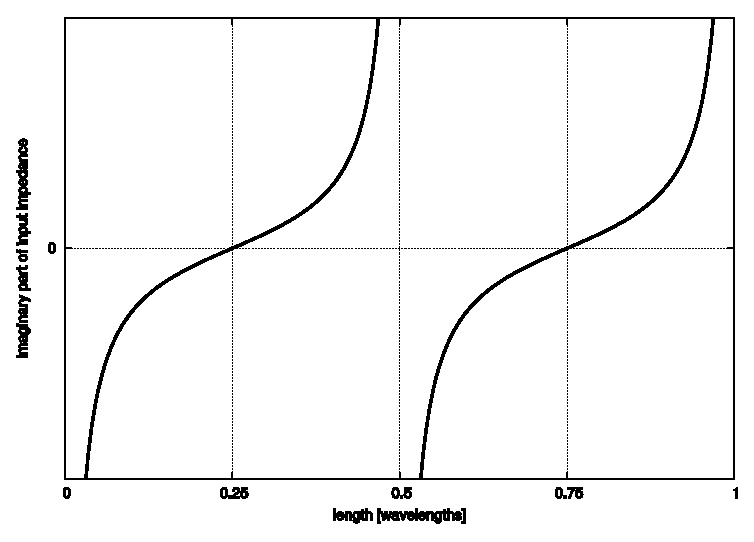
\includegraphics[width=\columnwidth]{modules/m0088_fZinOC.eps}
}}{A plot of the imaginary part of the input impedance (no scale shown) versus length from zero to 1 wavelength.  The plot has the form of the cotangent function, with zeros at 0.25 and 0.75 wavelengths and positive asymptotes at 0.5 and 1 wavelengths.}\\
(b) Open-circuit termination ($Z_L\rightarrow\infty$).
\end{center} 
\caption{\label{m0088_fZin}Input reactance (Im$\left\{Z_{in}\right\}$) of a stub. Re$\left\{Z_{in}\right\}$ is always zero.}
\end{figure}

%------------------------------------------------

For an open circuit 
\index{open circuit}
\index{stub!open circuit}
termination, $Z_L\rightarrow\infty$, $\Gamma=+1$, and we find 
%
\begin{flalign}
Z_{in}(l) &= Z_0 \frac{ 1 + \Gamma e^{-j2\beta l} }{  1 - \Gamma e^{-j2\beta l} } \nonumber \\
          &= Z_0 \frac{ 1 + e^{-j2\beta l} }{  1 - e^{-j2\beta l} } 
\end{flalign}
%
Following the same procedure detailed above for the short-circuit case, we find
%
\begin{equation}
\boxed{
Z_{in}(l) = -jZ_0 \cot \beta l
}
\label{m0088_eZstubOC}
\end{equation}

Figure~\ref{m0088_fZin}(b) shows the result for open-circuit termination.
As expected, $Z_{in}\rightarrow\infty$ for $l=0$, and the same $\lambda/2$ periodicity is observed.
What is of particular interest now is that at $l=\lambda/4$ we see $Z_{in}=0$. In this case, the transmission line has transformed the \emph{open} circuit termination into a \emph{short} circuit.  

Now taking stock of what we have determined:

%ORB HIGHLIGHT
\begin{mdframed}[backgroundcolor=yellow!20,nobreak=true] 
The input impedance of a short- or open-circuited lossless transmission line is completely imaginary-valued and is given by Equations~\ref{m0088_eZstubSC} and \ref{m0088_eZstubOC}, respectively. 
\end{mdframed}

%ORB HIGHLIGHT
\begin{mdframed}[backgroundcolor=yellow!20,nobreak=true] 
The input impedance of a short- or open-circuited lossless transmission line alternates between open- ($Z_{in}\rightarrow\infty$) and short-circuit ($Z_{in}=0$) conditions with each $\lambda/4$-increase in length. 
\end{mdframed}

{\bf Additional Reading:}
\begin{itemize}
\item ``\href{https://en.wikipedia.org/wiki/Stub_(electronics)}{Stub (electronics)}'' on Wikipedia.
\end{itemize}

\index{transmission line!input impedance|)}
